\chapter{IEEE 802.15.4}
\noindent

\section{Apresentação do protocolo}

\paragraph{}	O protocolo IEEE 802.15.4 é um padrão que define redes de área pessoal sem fio de baixas taxas (LR-WPAN), porém há implementações do protocolo que extravasam o limite de alcance de uma rede pessoal, assim podendo ser considerada como WAN. Ele especifica principalmente a camada física e a subcamada MAC, e pode operar com o IPv6.


\section{Escolha do IEEE 802.15.4}

\paragraph{}	Como o objetivo do projeto é fazer uma rede Ad Hoc com sistemas embarcados em VANTs, será muito importante que a rede ofereça recursos de escalabilidade, longa duração de bateria e confiabilidade. Requisitos encontrados no protocolo IEEE 802.15.4.

\paragraph{}	Além desses motivos, o IEEE 802.15.4 tem implementações comerciais de sucesso como o \textit{ZigBee}, que tem sido, constantemente, apresentado em diversos artigos acadêmicos \citep{CUNY} \citep{pfcmelhorqueonosso}- fatores que indicam a aplicabilidade desse protocolo.  

\section{Camadas do Modelo OSI no IEEE 802.15.4}
\subsection{Camada Física}
\paragraph{} A camada física (PHY) é responsável pela interface do meio de transmissão com a subcamada MAC. No protocolo IEEE 802.15.4 a camada física tem como funções principais a escolha de canais, sincronização de pacotes, modulação e demodulação. Além destas funções, a camada física provê mecanismos para passar e receber dados da subcamada MAC \citep{IEEE2016}. 

\subsubsection{Gerenciamento de Canais}
\paragraph{} O IEEE 802.15.4 trabalha em três bandas de frequências diferentes, centradas em 868 Mhz, 915 MHz e 2400 MHz. As bandas tem: 1, 10 e 16 canais respectivamente, conforme mostra a figura \ref{fig:figura3}.

\begin{figure}[!ht]
	\centering
	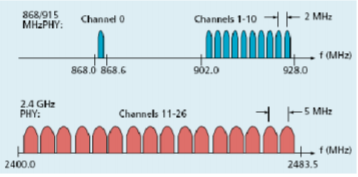
\includegraphics[width=0.5\textwidth]{Figuras/canais.PNG}   
	\caption{Canais do IEEE 802.15.4. \citep{Ufes}}
	\label{fig:figura3}
\end{figure}

\paragraph{} Para a escolha de canal, é feita uma varredura em uma determinada banda de frequência, permitindo que camadas superiores selecionem o canal apropriado. 

\paragraph{} O principal critério de escolha é pela detecção de energia, assim sendo, o canal de menor energia será o escolhido. Para isso o protocolo dispõe de um detector de energia que fornece, com um inteiro de 8 bits, o valor de potência do canal de até 10 dB acima da sensibilidade do receptor.

\paragraph{} A fim de eliminar interferências de outras redes, o IEEE 802.15.4 impõe um regime de rejeição de canais.

\paragraph{} Ao receber um sinal, o canal deve ser rejeitado,  caso haja um outro sinal do mesmo nível, ou mais fraco em um canal adjacente, ou ainda, um sinal de no máximo 24 dB mais forte em um canal alternado.

\subsubsection{Estrutura dos pacotes}

\paragraph{} Na camada física do IEEE 802.15.4,
 o pacote é dividido em 4 partes: preâmbulo, delimitador, cabeçalho e PHY \textit{Service Data Unit} (PSDU). Essa estrutura é representada pela figura \ref{fig:figura4}:
 
 \begin{figure}[!ht]
	\centering
	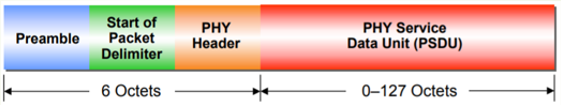
\includegraphics[width=0.5\textwidth]{Figuras/pacote_PHY.PNG}   
	\caption{Modelo de pacote da camada física. \citep{EATON}}
	\label{fig:figura4}
\end{figure}

 
 \paragraph{} O preâmbulo é constituído de 4 bytes que tem como principal função o treinamento do equalizador. A modulação que está sendo usada na transmissão será indicada por uma sequência de bits. No caso deste projeto, o padrão de cada byte será "01010101", que caracteriza o GFSK.
 
 \paragraph{} O delimitador (\textit{Start of Packet Delimeter}) são 8 bits pré-estabelecidos para indicar o final do preâmbulo e atua como um sincronizador. Para o IEEE 802.15.4 essa sequência será "11100101".
 
 \paragraph{} Cabeçalho PHY (PHR) é definido por apenas por 1 byte. Esse byte é constituído por 7 bits para definir o tamanho da PSDU e o oitavo bit é reservado.
 
 \paragraph{} O PSDU é o \textit{payload} da camada física e o seu tamanho pode variar de 0 à 127 bytes.
 
 \subsubsection{Parâmetros para o projeto}
 \paragraph{} O padrão IEEE 802.15.4 para a modulação GFSK utiliza os seguintes parâmetros (tabela \ref{tab:tabela1}):
 
\begin{table}[ht]
\centering
\caption{Parâmetros do IEEE 802.15.4 usados no projeto.}
\vspace{0.5cm}
\begin{tabular}{r|lr}
 
Modulação & GFSK \\
\hline
Banda de operação & 920 MHz \\
Taxa de bits & 100 kbps (100 kbauds) \\
Tamanho do canal & 2 Mhz \\
Potência de transmissão & Pelo menos -3 dBm \\
Sensibilidade do receptor & -85 dBm \\
Número de canais & 10 \\
Largura de banda & 2000 KHz 
 
\end{tabular}
\label{tab:tabela1}
\end{table}
 
\subsubsection{Modulação}
\paragraph{} O protocolo IEEE 802.15.4 permite o uso de diversas modulações, porém a modulação utilizada pelo rádio nRF24l01+ é a GFSK (\textit{Gaussian frequency-shift keying}).

\paragraph{} Essa modulação consiste no chaveamento deslocado de frequência binário com um filtro gaussiano na entrada do sistema. A consequência desse processo é a filtragem dos pulsos de dados para tornar as transições mais suaves. Sua principal vantagem é a redução da potência da banda lateral, assim reduzindo a interferência entre canais vizinhos. O protocolo utiliza um filtro cujo BT é de 0,5 e o índice de modulação do sinal é unitário.

\begin{figure}[!ht]
    \centering
    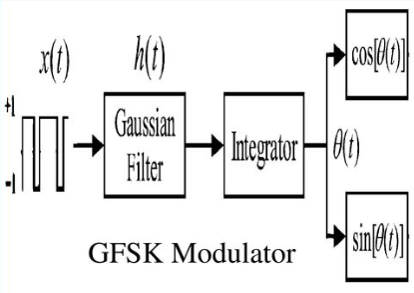
\includegraphics[width=0.4\textwidth]{Figuras/GFSK1.PNG}
    \caption{Diagrama de blocos da modulação GFSK. \citep{IEEE2015}}
    \label{fig:figura5}
\end{figure}
    
\begin{figure}[!ht]
    \centering
    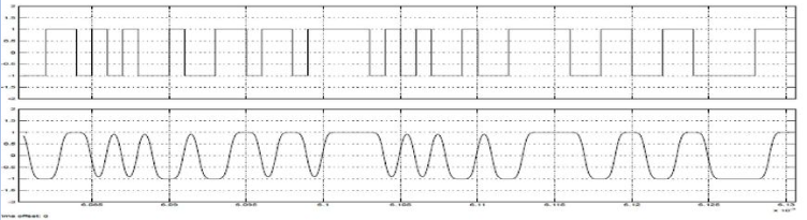
\includegraphics[width=0.6\textwidth]{Figuras/GFSK2.PNG}
    \caption{Comparação das modulações GFSK e FSK. \citep{IEEE2015}}
    \label{fig:figura6}
\end{figure}

\paragraph{} Para melhor funcionamento da modulação, o protocolo faz uso obrigatório \textit{Data Whitening}. Esse processo se fundamenta na descorrelação entre os bits a serem enviados, visando evitar sequências longas de bits iguais. 
 
\paragraph{} O \textit{Data Whitening} é o resultado do "ou exclusivo" entre os bits de entrada com pseudo-ruído de 9 bits gerado pelo mecanismo da figura \ref{fig:figura7}: 

\begin{figure}[!ht]
	\centering
	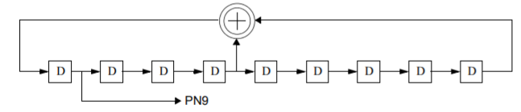
\includegraphics[width=0.5\textwidth]{Figuras/PN9.PNG}   
	\caption{Mecanismo de pseudo ruído de 9 bits. \citep{IEEE2015}}
	\label{fig:figura7}
\end{figure}

\paragraph{} Onde PN9 é a sequência definida pelo algoritmo da figura, com semente “111111111”.


\subsection{Subcamada MAC}
\paragraph{} A subcamada MAC é a parte inferior da camada de enlace, que fornece acesso às camadas superiores.

\paragraph{} Entre as suas principais funcionalidades estão a associação e desassociação de dispositivos na rede e o controle de acesso a canais associados. 

\paragraph{}Além dessas funções, a subcamada MAC é responsável por gerar \textit{beacons} de rede que permitem que os dispositivos localizem uma rede existente ou, no caso de redes TDMA, que forneçam uma indicação de tempo para os dispositivos clientes acessarem o canal durante períodos baseados em contenção e sem contenção.

\paragraph{} Para as camadas superiores, a subcamada MAC também oferece serviços de encaminhamento de dados destinados ou oriundos das camadas superiores (MCPS), e de mecanismo para controlar as configurações de comunicação, de rádio e funcionalidade de rede, da camada acima (MLME)\citep{IEEE2016}.

%\subsubsection{Channel Hopping}
%\paragraph{} Channel Hopping pelo dicionário da IEEE Standards significa alternar periodicamente o canal usando uma sequência conhecida tanto para envio como para recebimento dispositivos onde o quadro inteiro é enviado em um único canal. 

%\paragraph{} Os dispositivos podem saltar 

\subsubsection{Operação com \textit{Beacon}}
\paragraph{} Toda rede IEEE 802.15.4 usa \textit{beacons} de um coordenador ao unir dispositivos à rede. Nessa operação, o coordenador envia uma sequência de sinais de \textit{beacon}, contendo informações, que permitem que os nós da rede sincronizem suas comunicações. 

\paragraph{} Dois \textit{beacons} consecutivos costumam marcar o início e o fim de um superquadro. Um superquadro é uma estrutura de 16 intervalos de tempo que podem ser usados para comunicação.

\paragraph{} Um superquadro pode ser dividido em duas partes: Uma é a parte inativa que permite o coordenador entrar em modo de baixa potência; a outra, é a parte ativa que apresenta dois períodos principais o CAP (\textit{Contention access period}) e o CFP (\textit{Contention free period}). Conforme mostra a figura \ref{fig:figura8}:

\begin{figure}[!ht]
	\centering
	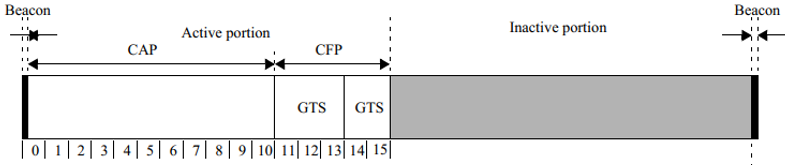
\includegraphics[width=0.6\textwidth]{Figuras/superquadro.PNG}   
	\caption{Estrutura de um Superquadro. \citep{IEEE2015}}
	\label{fig:figura8}
\end{figure}

\paragraph{} Durante o CAP, todos os quadros, com exceção dos quadros de ACK, usarão o mecanismo do CSMA/CA (descrito no tópico 3.3.2.2) para acessar o canal. Entre duas transmissões de quadro no CAP, a subcamada MAC exige um período entre quadros (IFS) para poder processar o último quadro enviado. 

\paragraph{} Ao contrário do CAP, as transmissões feitas dentro do CFP não utilizam CSMA/CA. Além disso, dentro do CFP ocorrem os GTS (\textit{Guaranteed Time Slot}), que são \textit{slots} do superquadro dedicados à comunicação entre um dispositivo e o coordenador da PAN. No superquadro podem haver até 7 GTSs.

\subsubsection{CSMA/CA}
\paragraph{} O CSMA/CA (Acesso múltiplo com verificação de portadora com prevenção de colisão) é um método de acesso múltiplo no qual a portadora, antes de iniciar a transmissão, escuta o canal e envia os dados, se esse estiver inativo; porém, se o canal estiver ocupado, a portadora aguardará, por um tempo aleatório, para a retransmissão.

\paragraph{} Para evitar o problema do terminal oculto, o CSMA/CA utiliza-se de pequenos pacotes chamados RTS (\textit{Ready to send}) e CTS (\textit{Clear to send}). O RTS é o pedido do terminal para poder realizar a transmissão, porém, só poderá enviar os pacotes após receber do ponto de acesso o CTS. Esse processo é eficiente pelo ponto de vista de que só poderá haver um CTS enquanto o canal estiver desocupado, porém essa prática pode congestionar o canal, se for utilizada em excesso \citep{Tanenbaum}.  

\paragraph{} Por conta de diversos terminais poderem ver o ponto de acesso e, pela dificuldade de se ouvir outras transmissões na rede, devido a longas distâncias, o método do CSMA/CA se tornou ideal para a rede ad hoc sem fio, que foi proposta, para este projeto.

\paragraph{} O IEEE 802.15.4 oferece diversos algoritmos de acesso randômico, porém o escolhido para o projeto foi o CSMA/CA com o fluxograma, conforme a figura \ref{fig:figura9}, onde "sucesso" representa a permissão para começar a transmissão, conforme a figura 3.7:

\begin{figure}[!ht]
	\centering
	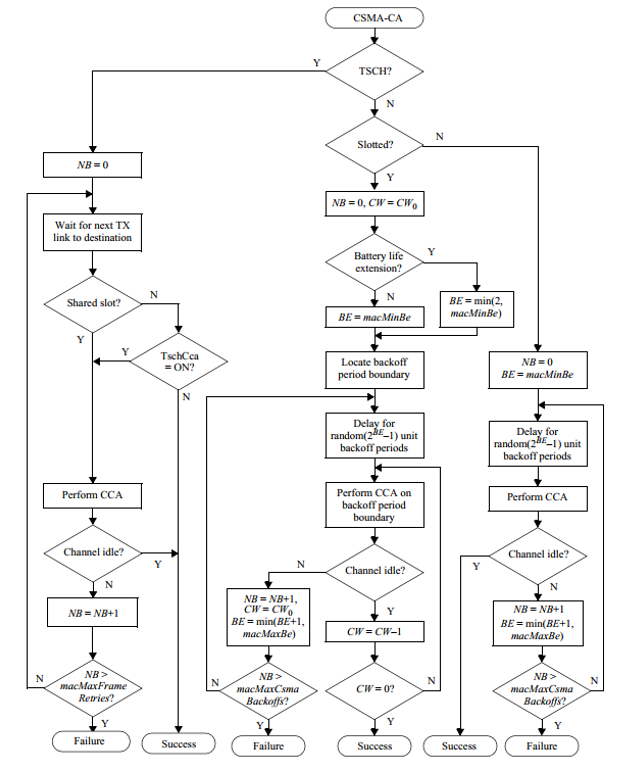
\includegraphics[width=0.6\textwidth]{Figuras/fluxograma_CSMA.PNG}   
	\caption{Fluxograma CSMA/CA do IEEE 802.15.4. \citep{IEEE2015}}
	\label{fig:figura9}
\end{figure}


\newpage
\subsubsection{Estrutura dos Pacotes}
\paragraph{} O pacote da subcamada MAC se encontra dentro da PSDU e é subdividida em três partes principais: MAC \textit{header} (MHR), MAC \textit{payload} e MAC \textit{footer} (MFR). Conforme mostram as figuras \ref{fig:figura10} e \ref{fig:figura11}:


\begin{figure}[!ht]
    \centering
    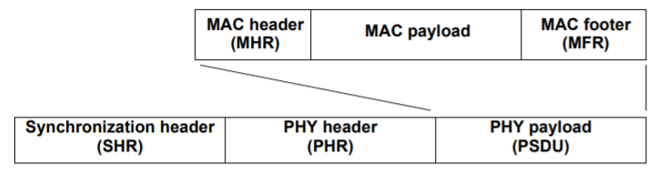
\includegraphics[width=0.6\textwidth]{Figuras/MAC1.PNG}
    \caption{Pacote MAC em relação à camada física. \citep{IEEE2015}}
    \label{fig:figura10}
\end{figure}
    
\begin{figure}[!ht]
    \centering
    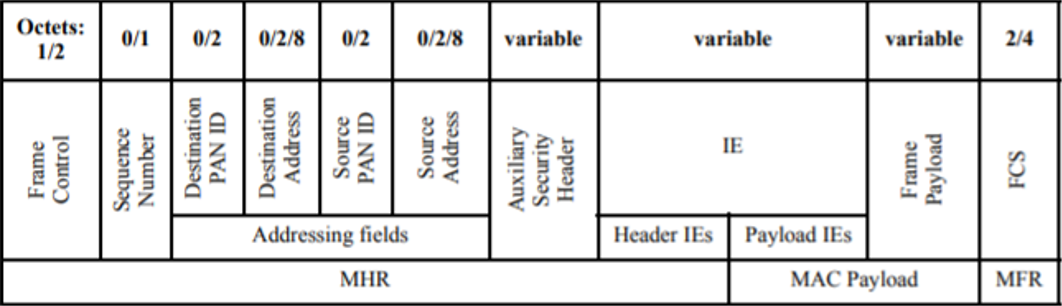
\includegraphics[width=0.6\textwidth]{Figuras/MAC2.PNG}
    \caption{Divisão do pacote da subcamada MAC. \citep{IEEE2015}}
    \label{fig:figura11}
\end{figure}

\paragraph{}A primeira parte do MHR é o \textit{Frame Control}, que é responsável por diversas configurações da transmissão. Uma dessas configurações é a definição do tipo do pacote. São usados os 3 primeiros bits para dizer se o pacote é um \textit{beacon}, se é de dados, de \textit{acknowledgment}, entre outros. O bit seguinte é o de habilitação de segurança, o qual não será habilitado para o projeto. Depois, vem o bit de pendência, que é enviado pelo dispositivo, caso tenha mais dados do que um único pacote permite. A seguir vem o AR (\textit{ACK request}) que especifica se é necessário um quadro de confirmação do receptor. O sétimo bit do \textit{Frame Control} é o de compressão do PAN ID. O oitavo e nono bits são respectivamente os indicativos de supressão do número de sequência e de presença do IE (\textit{Information Element}), ambos serão ausentes no pacote gerado para o projeto. Os dois bits do \textit{Destination Addressing Mode} e do \textit{Sorce Addressing Mode} serão "10" para endereços de 16 bits e "11" para endereços de 64 bits. Por fim, o \textit{Frame Control} especifica a versão do protocolo IEEE 802.15.4 que será usada no quadro sendo: "00" para a versão de 2003, "01" para a de 2006 e "10" para a atual. O \textit{Frame Control} pode ser melhor visualizado pela figura \ref{fig:figura12}: 

\begin{figure}[!ht]
	\centering
	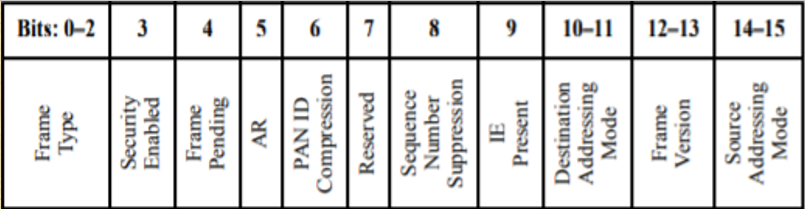
\includegraphics[width=0.6\textwidth]{Figuras/frame_control.PNG}   
	\caption{Divisão do campo \textit{Frame Control}. \citep{IEEE2015}}
	\label{fig:figura12}
\end{figure}

\paragraph{} Os campos de PAN ID, do destino e da fonte, apresentam um tamanho de 2 bytes, enquanto os endereços podem variar entre curtos (2 bytes) ou longos (8 bytes), de acordo com o especificado no \textit{Frame Control}.   

\paragraph{} As demais subdivisões do MHR, como o Número de sequência, o Cabeçalho de Segurança Auxiliar e o Elemento de Informação serão suprimidas no pacote do projeto, portanto, não serão abordados neste texto.

\paragraph{} O MAC \textit{Payload} será constituído por dados de informação e seu tamanho é variável de acordo com o tamanho do PSDU especificado na camada física.

\paragraph{} O MAC \textit{footer} contém CRC de 16 ITU-T e 32 bits equivalente ao ANSI X3.66-1979, e é formado pelo polinômio binário correspondente ao resto da divisão da sequência de bits do MHR e MAC \textit{payload} pelo polinômio gerador.

\paragraph{} Como o rádio nrf24l01+ permite no máximo de 16 bits de CRC, o polinômio gerador usado no projeto será de acordo com a seguinte forma:

\begin{equation}
    G_{16}(x) = x^{16} + x^{12} + x^5 + 1 
\end{equation}

\subsubsection{Rejeição de Pacotes}
\paragraph{} A subcamada MAC é capaz de filtrar os quadros recebidos de forma que só restem os quadros que são de interesse para a camada superior.

\paragraph{} O primeiro nível de filtragem ocorre quando os valores do MAC \textit{footer} estiverem incorretos. Como esse campo é de verificação de erros, qualquer pacote que tiver erro não será passado para a camada superior.

\paragraph{} O próximo nível de filtragem dependerá se o MAC estiver em modo promíscuo, neste caso, o pacote não receberá nenhum filtro após a primeira filtragem. Se não tiver em modo promíscuo, a próxima análise consiste em verificar se a subcamada está operando em varredura. Durante uma varredura, a subcamada MAC deve descartar todos os quadros recebidos pelo serviço de dados PHY.

\paragraph{} Por fim, será filtrado todo quadro que não contiver um tipo ou versão do protocolo. 

\subsubsection{6LoWPAN}
\paragraph{} O padrão IEEE 802.15.4 utiliza o IPv6 como protocolo de endereçamento, porém o IPv6 tem um tamanho de pacote maior que os 128 bytes disponíveis no PSDU. Para resolver esse problema, foi criado o 6LoWPAN (\textit{IPv6 in Low-Power Wireless Personal Area Networks Groups})\citep{6lowpan}.

\paragraph{} O 6LoWPAN foi uma solução da IETF para a adaptação do pacote IPv6 ao IEEE 802.15.4. Essa compressão de pacote permite dispositivos com baixo poder computacional usar a mais nova versão do protocolo IP. Para a realização da compressão, o 6LoWPAN utiliza de informações de protocolos de outras camadas.   

\paragraph{}Essa seção é baseada no padrão escrito pela IEEE-SA Standart Board \citep{IEEE2015}

\section{\textit{OpenThread}}
\subsection{O que é \textit{OpenThread}}
\paragraph{} \textit{OpenThread} é uma implementação do código do protocolo de rede \textit{Thread} feito pela Nest (uma empresa do grupo Google). A Nest trabalha na área de tecnologia para automação de serviços domésticos como termostatos via wi-fi, detectores de fumaça e sistemas de segurança programáveis. Para o funcionamento desses produtos, foi necessário o uso do protocolo \textit{Thread}, que é uma tecnologia de rede \textit{mesh} de baixo consumo, baseada em IPv6 \citep{Open}. 

\paragraph{} O \textit{OpenThread} implementa as camadas de rede \textit{Thread} como a do IEEE 802.15.4, e tem como principais recursos a segurança, com autenticação dos dispositivos de rede e criptografia das comunicações, confiabilidade, eficiência em relação ao consumo de energia e escalabilidade da rede. O \textit{OpenThread} trabalha com a versão de 2006 do IEEE 802.15.4. 

\subsection{Funções do \textit{Openthread}}
\paragraph{} Na rede \textit{Thread} existem duas funções de encaminhamento: o roteador e o dispositivo final (ED). Conforme mostra a figura \ref{fig:figura13}:

\begin{figure}[!ht]
	\centering
	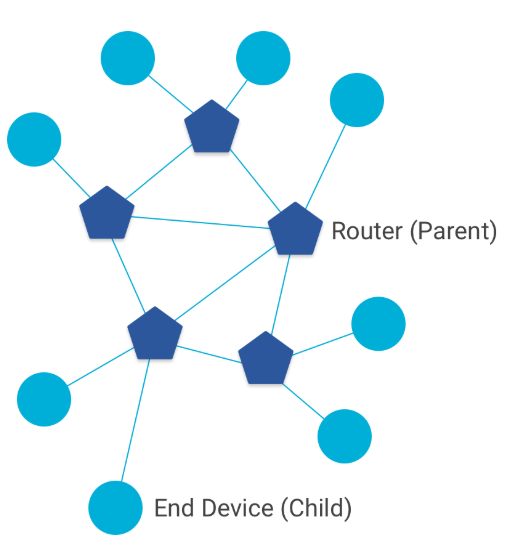
\includegraphics[width=0.4\textwidth]{Figuras/openthread.PNG}   
	\caption{Exemplo de rede Thread. \citep{Open}}
	\label{fig:figura13}
\end{figure}

\paragraph{}O roteador é um nó que encaminha pacotes para os dispositivos da rede, além de introduzir de forma segura novos dispositivos nela. Já o dispositivo final, não encaminha pacotes para outros dispositivos de rede, pois se comunica, principalmente, com um único roteador.
O protocolo \textit{Thread} nomeia a relação do roteador com o dispositivo final de relacionamento pai-filho, onde o roteador é o pai e o ED é o filho.

\paragraph{} Numa rede, pode acontecer de um roteador não ter filhos, então ele pode ser rebaixado e operar como um dispositivo final. O mesmo pode acontecer com um ED que ao ser o único nó ao alcance de um novo dispositivo que deseja ingressar na rede, ele pode operar como um roteador.

\paragraph{} Na rede \textit{Thread} existem também o \textit{Thread} Líder e o Roteador de borda. O \textit{Thread} Líder é o roteador responsável por gerenciar o conjunto de roteadores na rede, ele é dinamicamente auto-eleito e distribui informações de configuração em toda a rede. O Roteador de borda é um dispositivo que pode encaminhar informações para uma rede externa não \textit{Thread}.

\paragraph{} A rede \textit{Thread} permite apenas um líder, 32 roteadores e 511 dispositivos finais, por roteador.

\subsection{Endereçamento IPv6}
\paragraph{} Para fazer o endereçamento, primeiramente o \textit{Thread} gera um localizador de roteamento (RLOC). Esse localizador é gerado de forma que cada roteador mantenha uma tabela de todos os seus filhos, cuja combinação (ID do roteador + 0 + ID do filho) identifica de forma exclusiva um dispositivo dentro da topologia, então cada dispositivo terá um RLOC diferente. Como todos os dispositivos recebem uma ID, o RLOC de 16 bits gerado, quando os IDs do roteador e do filho forem iguais a 1, será segundo a figura \ref{fig:figura14}. O RLOC de 16 bits do roteador será gerado da mesma forma, só que o ID do filho será igual a zero;

\begin{figure}[!ht]
	\centering
	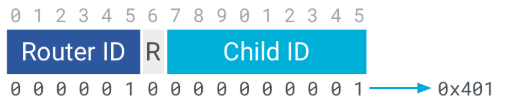
\includegraphics[width=0.5\textwidth]{Figuras/RLOC16.PNG}   
	\caption{Exemplo de localizador de roteamento de 16 bits. \citep{Open}}
	\label{fig:figura14}
\end{figure}

\paragraph{} Esse localizador de roteamento, faz parte do identificador de interface (IID), que corresponde aos últimos 64 bits do endereço IPv6. Então o IID é sempre do tipo 0000:00ff:fe00:RLOC16.

\paragraph{} Por fim, o RLOC completo será a combinação do prefixo local de malha com o IID. Dessa forma, o RLOC representa um dos tipos de endereço \textit{unicast} IPv6 que um dispositivo \textit{Thread} pode ter.

\subsection{Criação de Redes}
\paragraph{} Para que um dispositivo se junte a uma rede ou crie uma rede própria, é preciso que ele transmita um \textit{Beacon request}, em um canal específico para todo seu alcance. Um outro dispositivo, ao receber essa solicitação, responde com um \textit{beacon} que contém seu PAN ID, XPAN ID, bem como o Nome da Rede. Esse processo é realizado para todos os canais, assim podendo se conectar a uma rede ou criar uma rede própria.

\paragraph{} O \textit{Mesh Link Establishment} (MLE) é o protocolo que vai configurar os enlaces e disseminar as informações sobre a rede. Esse protocolo fornece informações do tipo: Dados do líder, dados de rede e propagação das rotas.

\paragraph{}Para criar uma nova rede, um dispositivo terá que selecionar o canal menos ocupado, além de um PAN ID que não esteja em uso. Após esse processo, ele se declarará líder e envia mensagens de informações MLE para os outros dispositivos 802.15.4.

\subsection{Seleção de Roteador} 
\paragraph{} Conjunto Dominante Conectado é um sistema que garante um nível mínimo de redundância para a rede. Para isso, tem que haver apenas um caminho de roteadores entre dois roteadores. Todos os roteadores poderão se comunicar, e cada dispositivo final deverá estar conectado diretamente a um roteador.

\paragraph{} O número de roteadores em uma rede \textit{Thread} é variável, de acordo com as suas necessidades. Roteadores devem ser adicionados, para aumentar a cobertura, aumentar a diversidade de caminhos, manter redundância e conectar mais dispositivos finais. A remoção se faz necessária, para reduzir o estado de roteamento, e permitir novos roteadores em outras redes. 
